\documentclass[a4paper,10pt]{report}
% \usepackage[utf8]{inputenc}
% \usepackage{jheppub} 
\usepackage[T1]{fontenc}
\usepackage{booktabs}
\usepackage[dvips,table]{xcolor} 
\usepackage{amsmath}
\usepackage{xspace}
\usepackage{dcolumn}
\usepackage{hyperref}
\usepackage{tabularx}
\usepackage{graphicx}
\usepackage{caption}
\usepackage
[subrefformat=parens,position=top,skip=-15pt,margin=15pt,justification=justified,singlelinecheck=false]
{subcaption}


\renewcommand{\topfraction}{1}
\renewcommand{\bottomfraction}{1}
\setcounter{topnumber}{2}
\setcounter{bottomnumber}{2}
\setcounter{totalnumber}{4}    
\renewcommand{\textfraction}{0.07}
\renewcommand{\floatpagefraction}{0.9}

\newcommand{\eq}[1]{\begin{equation} #1 \end{equation}}
\newcommand{\eqa}[1]{\begin{eqnarray} #1 \end{eqnarray}}

\setlength{\clubpenalty}{10000}
\setlength{\widowpenalty}{10000}
\setlength{\displaywidowpenalty}{10000}
% \allowdisplaybreaks[1]

\newcommand{\Pl}{\ell}
\newcommand{\fb}{{\ensuremath\unskip\,\text{fb}}\xspace}
% % new commands for cross referencing
\def\refeq#1{\mbox{(\ref{#1})}}
\def\reffi#1{\mbox{Figure~\ref{#1}}}
\def\reffis#1{\mbox{Figures~\ref{#1}}}
\def\refta#1{\mbox{Table~\ref{#1}}}
\def\reftas#1{\mbox{Tables~\ref{#1}}}
\def\refse#1{\mbox{Section~\ref{#1}}}
\def\refapp#1{\mbox{App.~\ref{#1}}}
\def\citere#1{\mbox{Ref.~\cite{#1}}}
\def\citeres#1{\mbox{Refs.~\cite{#1}}}

\newcommand{\ri}{\mathrm i}

\newcommand{\ie}{\emph{i.e.}\ }
\newcommand{\eg}{\emph{e.g.}\ }

\def\be{\begin{equation}}
\def\ee{\end{equation}}

\newcommand{\qqb}{\ensuremath{q\bar{q}}\xspace}
\newcommand{\PH}{\ensuremath{\text{H}}\xspace}
\newcommand{\Pj}{\ensuremath{\text{j}}\xspace}
\newcommand{\Pp}{\ensuremath{\text{p}}\xspace}
\newcommand{\Pe}{\ensuremath{\text{e}}\xspace}
\newcommand{\Pb}{\ensuremath{\text{b}}\xspace}
\newcommand{\Pq}{\ensuremath{\text{q}}\xspace}
\newcommand{\Pt}{\ensuremath{\text{t}}\xspace}
\newcommand{\Pu}{\ensuremath{\text{u}}\xspace}
\newcommand{\Pd}{\ensuremath{\text{d}}\xspace}
\newcommand{\Ps}{\ensuremath{\text{s}}\xspace}
\newcommand{\Pc}{\ensuremath{\text{c}}\xspace}
\newcommand{\Pg}{\ensuremath{\text{g}}\xspace}
\newcommand{\Pw}{\ensuremath{\text{w}}\xspace}
\newcommand{\PW}{\ensuremath{\text{W}}\xspace}
\newcommand{\PZ}{\ensuremath{\text{Z}}\xspace}
\newcommand{\Pbj}{\ensuremath{\text{j_b}}\xspace}
                                    
\newcommand{\Mt}{\ensuremath{m_\Pt}\xspace}
\newcommand{\MH}{\ensuremath{M_\PH}\xspace}
\newcommand{\MWOS}{\ensuremath{M_\PW^\text{OS}}\xspace}
\newcommand{\MW}{\ensuremath{M_\PW}\xspace}
\newcommand{\MZOS}{\ensuremath{M_\PZ^\text{OS}}\xspace}
\newcommand{\MZ}{\ensuremath{M_\PZ}\xspace}
\newcommand{\Mb}{\ensuremath{m_\Pb}\xspace}
\newcommand{\Gt}{\ensuremath{\Gamma_\Pt}\xspace}
\newcommand{\GH}{\ensuremath{\Gamma_\PH}\xspace}
\newcommand{\GZ}{\ensuremath{\Gamma_\PZ}\xspace}
\newcommand{\GZOS}{\ensuremath{\Gamma_\PZ^\text{OS}}\xspace}
\newcommand{\GW}{\ensuremath{\Gamma_\PW}\xspace}
\newcommand{\GWOS}{\ensuremath{\Gamma_\PW^\text{OS}}\xspace}

\newcommand{\MeV}{\ensuremath{\,\text{MeV}}\xspace}
\newcommand{\GeV}{\ensuremath{\,\text{GeV}}\xspace}
\newcommand{\TeV}{\ensuremath{\,\text{TeV}}\xspace}

\newcommand{\alphas}{\ensuremath{\alpha_\text{s}}\xspace}
\newcommand{\order}[1]{\ensuremath{\mathcal{O}{\left(#1\right)}}\xspace}

\newcommand{\abs}[1]{\left|#1\right|}
\newcommand{\deltar}{\ensuremath{\Delta R}\xspace}

\newcommand{\GF}{\ensuremath{G_\mu}}

\newcommand{\pt}{\ensuremath{p_\text{T}}\xspace}
\newcommand{\ptsub}[1]{\ensuremath{p_{\text{T},#1}}\xspace}
\newcommand{\etsub}[1]{\ensuremath{E_{\text{T},#1}}\xspace}

\renewcommand{\Re}{\mathop{\mathrm{Re}}\nolimits}
\renewcommand{\Im}{\mathop{\mathrm{Im}}\nolimits}

\newcommand{\MVOS}{\ensuremath{M_{V}^\text{OS}}\xspace}%
\newcommand{\GVOS}{\ensuremath{\Gamma_{V}^\text{OS}}\xspace}%

\newcommand{\sq}{\tilde{q}}
\newcommand{\su}{\tilde{u}}
\newcommand{\sd}{\tilde{d}}
\newcommand{\gl}{\tilde{g}}
\def\bom#1{{\mbox{\boldmath $#1$}}}
\newcommand\nn         {\nonumber}
\newcommand{\sul}{\tilde{u}_L}
\newcommand{\scl}{\tilde{c}_L}
\newcommand{\sdl}{\tilde{d}_L}
\newcommand{\ssl}{\tilde{s}_L}
\newcommand{\sur}{\tilde{u}_R}
%\newcommand{\scr}{\tilde{c}_R}
\newcommand{\sdr}{\tilde{d}_R}
\newcommand{\ssr}{\tilde{s}_R}
\newcommand{\stone}{\tilde{t}_1}
\newcommand{\sbone}{\tilde{b}_1}
\newcommand{\sttwo}{\tilde{t}_2}
\newcommand{\sbtwo}{\tilde{b}_2}
\newcommand{\neutone}{\tilde{\chi}^0_1}
\newcommand\sss{\mathchoice%
{\displaystyle}%
{\scriptstyle}%
{\scriptscriptstyle}%
{\scriptscriptstyle}%
}
\newcommand{\newc}{\newcommand}
% \newc{\be}{\begin{equation}}
% \newc{\ee}{\end{equation}}
\newc{\bi}{\begin{itemize}}
\newc{\ei}{\end{itemize}}
\newc{\benu}{\begin{enumerate}}
\newc{\eenu}{\end{enumerate}}
\newc{\bc}{\begin{center}}
\newc{\ec}{\end{center}}
\newc{\bfig}{\begin{figure}}
\newc{\efig}{\end{figure}}
\newc{\qbar}{\bar{q}}
\newc{\go}{\tilde{g}}
\newc{\PB}{\textsc{Powheg-Box}}
\newcommand\matB{{\cal B}}
\newcommand\matR{{\cal R}}
\newcommand\matV{{\cal V}}
\newcommand\matO{{\cal O}}
\newcommand\matF{{\cal F}}

\newcommand{\Recola}{{\sc Recola}\xspace}
\newcommand{\Sherpa}{{\sc Sherpa}\xspace}
\newcommand{\Rivet}{{\sc Rivet}\xspace}
\newcommand{\Amegic}{A\protect\scalebox{0.8}{MEGIC}\xspace}
\newcommand{\Comix}{C\protect\scalebox{0.8}{OMIX}\xspace}
\newcommand{\OpenLoops}{O\protect\scalebox{0.8}{PEN}L\protect\scalebox{0.8}{OOPS}\xspace}
\newcommand{\Njet}{N\protect\scalebox{0.8}{JET}\xspace}
\newcommand{\BlackHat}{B\protect\scalebox{0.8}{LACK}H\protect\scalebox{0.8}{AT}\xspace}
\newcommand{\Gosam}{G\protect\scalebox{0.8}{O}S\protect\scalebox{0.8}{AM}\xspace}
\newcommand{\mocanlo}{{\sc MoCaNLO}\xspace}
\newcommand{\collier}{{\sc Collier}\xspace}
\newcommand{\CutTools}{{\sc CutTools}\xspace}
\newcommand{\OneLOop}{{\sc OneLOop}\xspace}
\newcommand{\madgraph}{{\sc\small MadGraph5\_aMC@NLO}\xspace}
\newcommand{\madgraphbis}{{\sc\small MG5\_aMC@NLO}\xspace}
\newcommand{\rT}{{\mathrm{T}}}
\newcolumntype{.}{D{.}{.}{-1}}
\newcolumntype{d}[1]{D{.}{.}{#1}}

\renewcommand{\vec}[1]{\mathbf{#1}}
\colorlet{tableoverheadcolor}{gray!37.5}
\colorlet{tableheadcolor}{gray!25}
\colorlet{tablerowcolor}{gray!12.5}

\newcommand{\lsim}
{\;\raisebox{-.3em}{$\stackrel{\displaystyle <}{\sim}$}\;}
\newcommand{\gsim}
{\;\raisebox{-.3em}{$\stackrel{\displaystyle >}{\sim}$}\;}
\def\asymp#1{\;\raisebox{-.4em}{$\widetilde{\scriptstyle #1}$}\;}

\newlength{\width}
\newlength{\height}
\newcommand{\brabar}[1]{%
    \settoheight{\height}{\ensuremath{#1}}%
    \settowidth{\width}{\ensuremath{#1}}%
    \makebox[0pt][l]{\ensuremath{#1}}%
    \raisebox{1.26ex}{\scalebox{.3}{\textbf{(}}}%
    \rule[1.41\height]{0.7\width}{0.35pt}%
    \raisebox{1.26ex}{\scalebox{.3}{\textbf{)}}}%
}

% modifications for drafts for drafts
\newcommand{\mpar}[1]{{\marginpar{\hbadness10000%
                      \sloppy\hfuzz10pt\boldmath\bf\textcolor{red}{#1}}}%
                      \typeout{marginpar: #1}\ignorespaces}
\marginparwidth 1.2cm
\marginparsep 0.2cm
\def\draftdate{\relax}
\def\mda{\relax}
\def\mua{\relax}
\def\mla{\relax}
\def\draft{
\def\thtystars{******************************}
\def\sixtystars{\thtystars\thtystars}
\typeout{}
\typeout{\sixtystars**}
\typeout{* Draft mode!
         For final version remove \protect\draft\space in source file *}
\typeout{\sixtystars**}
\typeout{}
\def\draftdate{\today}
\def\mua{\marginpar[\boldmath\hfil$\uparrow$]%
                   {\boldmath$\uparrow$\hfil}\color{black}%
                    \typeout{marginpar: $\uparrow$}\ignorespaces}
\def\mda{\color{red}\marginpar[\boldmath\hfil$\downarrow$]%
                   {\boldmath$\downarrow$\hfil}%
                    \typeout{marginpar: $\downarrow$}\ignorespaces}
\def\mla{\marginpar[\boldmath\hfil$\rightarrow$]%
                   {\boldmath$\leftarrow $\hfil}%
                    \typeout{marginpar: $\leftrightarrow$}\ignorespaces}
\def\Mua{\marginpar[\boldmath\hfil$\Uparrow$]%
                   {\boldmath$\Uparrow$\hfil}\color{black}%
                    \typeout{marginpar: $\uparrow$}\ignorespaces}
\def\Mda{\color{red}\marginpar[\boldmath\hfil$\Downarrow$]%
                   {\boldmath$\Downarrow$\hfil}%
                    \typeout{marginpar: $\downarrow$}\ignorespaces}
\def\Mla{\marginpar[\boldmath\hfil\textcolor{red}{$\Rightarrow$}]%
                   {\boldmath\textcolor{red}{$\Leftarrow $}\hfil}%
                    \typeout{marginpar: $\leftrightarrow$}\ignorespaces}
\overfullrule 5pt
\oddsidemargin 15mm
\marginparwidth 29mm
}

% switch on draft mode
%\draft



% Title Page
\title{Monte Carlo comparisons \\
VBSCAN Cost Action}
\author{Mathieu Pellen, Marco Zaro, \\
Alexander Karlberg, Michael Rauch, J\"urgen Reuter}


\begin{document}
\maketitle

\begin{abstract}

\end{abstract}

\part{Introduction}

\part{$\Pp\Pp\to\mu^+\nu_\mu\Pe^+\nu_{\Pe}\Pj\Pj$}

\section{Input parameters}

- Centre-of-mass energy of $13\TeV$ at the LHC. \\
%
- Parton distribution function (PDF): NNPDF-3.0 at NLO with $\alpha_{\rm s} \left( \MZ \right) = 0.118$ (we use it at both LO and NLO). The
LHAPDF ID for this set is 260000.\\
%
- Flavour scheme: fixed $N_\text{F}=5$ flavour scheme ( no bottom quark appear in the final or initial state). 
This means that the bottom quark is considered massless. \\
%
- Photon induced are neglected (for now). \\
%
- Renormalisation scheme: complex-mass scheme if possible. If other schemes are used, we have to estimate the possible differences.
%
- Factorisation scheme: ${\overline{\rm MS}}$ as for NNPDF. \\
%
- Scales: factorisation and renormalisation scale, $\mu_R = \mu_F = \MW$. \\
%
- $\alpha$: $G_\mu$ scheme with:
%
\begin{equation}
  \alpha = \frac{\sqrt{2}}{\pi} G_\mu \MW^2 \left( 1 - \frac{\MW^2}{\MZ^2} \right)  \qquad \text{with}  \qquad   \GF    = 1.16637\times 10^{-5}\GeV.            
\end{equation}
%
The numerical value is: $\alpha = 7.555310522369 \times 10^{-3}$. \\
%
- Mass and width of the massive particles:
% 
\begin{alignat}{2}
                  \Mt   &=  173.21\GeV,       & \quad \quad \quad \Gt &= 0 \GeV,  \nonumber \\
                \MZOS &=  91.1876\GeV,      & \quad \quad \quad \GZOS &= 2.4952\GeV,  \nonumber \\
                \MWOS &=  80.385\GeV,       & \GWOS &= 2.085\GeV,  \nonumber \\
                M_{\rm H} &=  125.0\GeV,       &  \GH   &=  4.07 \times 10^{-3}\GeV.
\end{alignat}
%
The pole masses and widths entering the calculation are expressed in terms of the measured on-shell (OS) values for the W and Z bosons according to
%
\begin{equation}
        M_V = \MVOS/\sqrt{1+(\GVOS/\MVOS)^2}\,,\qquad  \Gamma_V = \GVOS/\sqrt{1+(\GVOS/\MVOS)^2}.
\end{equation}
%
Hence the numerical values are
\begin{alignat}{2}
                \MZ &=  91.1534806191827\GeV,      & \quad \quad \quad \GZ &= 2.494266378772824\GeV,  \nonumber \\
                \MW &=  80.3579736098775\GeV,       & \GW &= 2.084298998278219\GeV.
\end{alignat}
%
- Experimental signature:
two equally charged leptons, missing transverse energy and at least two jets. \\
- Clustering: QCD partons are clustered into jets using the anti-$k_\text{T}$ algorithm  with jet-resolution parameter $R=0.4$.
Photons from real radiation are recombined with the final-state quarks into jets or with the charged leptons into dressed leptons, in both cases via the anti-$k_\text{T}$ algorithm and a resolution parameter $R=0.1$ 
(this applies only when computing the EW corrections). \\
%
- Rapidity definition: $y=\frac{1}{2}\ln \frac{E+p_z}{E-p_z}$ where $E$ is the energy of the parton and $p_z$ the component of its momentum along the beam axis. \\
%
- Distance definition:
\begin{equation}
        \Delta R_{ij} = \sqrt{(\Delta \phi_{ij})^2+(\Delta y_{ij})^2},
\end{equation}
with $\Delta \phi_{ij}=\phi_i-\phi_j$ being the azimuthal-angle difference and $\Delta y_{ij} = y_i-y_j$ being the rapidity difference. \\
%
- Definition of the missing transverse energy: transverse momentum of the sum of the two neutrinos momenta. \\
%
- Cuts on the leptons:
\begin{align}
 \ptsub{\Pl} >  20\GeV,\qquad |y_{\Pl}| < 2.5, \qquad \Delta R_{\Pl\Pl}> 0.3.
\end{align}
%
- Missing energy cut:
\begin{align}
  \etsub{\text{miss}}=p_{\rm T, miss} >  40\GeV
\end{align}
%
- Jet definition:
%
\begin{align}
 \ptsub{\Pj} >  30\GeV, \qquad |y_\Pj| < 4.5 .
\end{align}
%
- Out of these 2/3 jets, the two hardest in pT (tagged jets)are required to have:
\begin{align}
 m_{\Pj \Pj} >  500\GeV,\qquad |\Delta y_{\Pj \Pj}| > 2.5.
\end{align}
%
- All jets in the event are required to satisfy 
\begin{align}
 \qquad\Delta R_{\Pj\Pl} > 0.3 .
\end{align}

\section{Codes}
\begin{table}
    \footnotesize
    \begin{tabularx}{\textwidth}{c|c|X|X|X|X|X}
        Contact person  &  Code  &  $\mathcal O(g_W^6)$ $s/t/u$  &  $\mathcal O(g_W^6)$ interf.  &  Off-shell  &  NF QCD  &  EW corr. to $\mathcal O(g_W^4g_s^2)$  \\
        \hline
        \hline
        A. Karlberg  &  {\sc POWHEG}  &  $t/u$  &  No  &  Yes  &  No  &  No  \\
        M. Pellen    &  {\sc Recola}  &  Yes  &  Yes  &  Yes  &  Yes  &  Yes  \\
        M. Rauch     &  {\sc VBFNLO}  &  Yes  &  No  &  Yes  &  No  &  No  \\
        C. Schwan    &   Private      &  $t/u$  &  No  &  Yes, virt. No  &  No  &  No  \\
        M. Zaro      &  {\sc MG5\_aMC}  &  Yes  &  Yes  &  Yes  &  No  &  No  
    \end{tabularx}
    \caption{\label{tab:codes} Summary of the different properties of the codes employed in the comparison.}
\end{table}

\subsection{ {\sc POWHEG}: Alexander Karlberg}
VBF approximation? \\
\subsection{ {\sc VBFNLO}: Michael Rauch}
VBF approximation \\
\subsection{ {\sc WHIZARD}: J\"urgen Reuter}
Full matrix element \\
\subsection{ \recola: Mathieu Pellen}
Full matrix element \\
\subsection{ \madgraph: Marco Zaro}
To be checked what is possible \\

\section{Observables}
- Cross section within cuts. \\
- Distribution in the number of jets. \\
- Invariant mass of the two hardest jets (two tagged jets). \\
$[0; 4\TeV]$ with bins of size $100\GeV$ (40 bins). \\
- $\ptsub{\Pj_1,\Pj_2}$ and $y_{\Pj_1,\Pj_2}$ of the two tagged jets (not their sum) \\
$\ptsub{\Pj_1,\Pj_2}$: $[0; 1\TeV]$ with bins of size $25\GeV$ (40 bins). \\
$y_{\Pj_1,\Pj_2}$: $[-5;5]$ with bins of size $0.5$ (20 bins). \\
- Invariant mass of the two charged leptons. \\
$[0; 4\TeV]$ with bins of size $100\GeV$ (40 bins). \\
- Zeppenfeld variable for $\mu^+$ and $\Pe^+$: \\
$z^*_\ell = |y_\ell - \left(y_{\Pj_1}+y_{\Pj_2} \right)/2|/|\Delta y_{\Pj\Pj}|$ \\
$[0;1.5]$ with bins of size $0.05$ (30 bins).

\section{Numerical results}

\subsection{LO $\mathcal{O}\left(\alpha^6\right)$}

\begin{table}[h!]
    \begin{tabular}{c|c}
        Code  &  $\sigma[\rm{fb}]$  \\
        \hline
        \hline
        {\sc POWHEG}  &  $1.5573 \pm 0.0003$ \\
        {\sc Recola}  &  $1.5503 \pm 0.0003$ \\
        {\sc VBFNLO}  &  $1.5538 \pm 0.0002$ \\
        Private       &  \\
        {\sc MG5\_aMC}&  $1.542 \pm 0.002$   
    \end{tabular}
    \caption{\label{tab:LOrates} LO rates within VBS cuts from the different codes.}
\end{table}

\begin{figure}[h!]
   \centering
   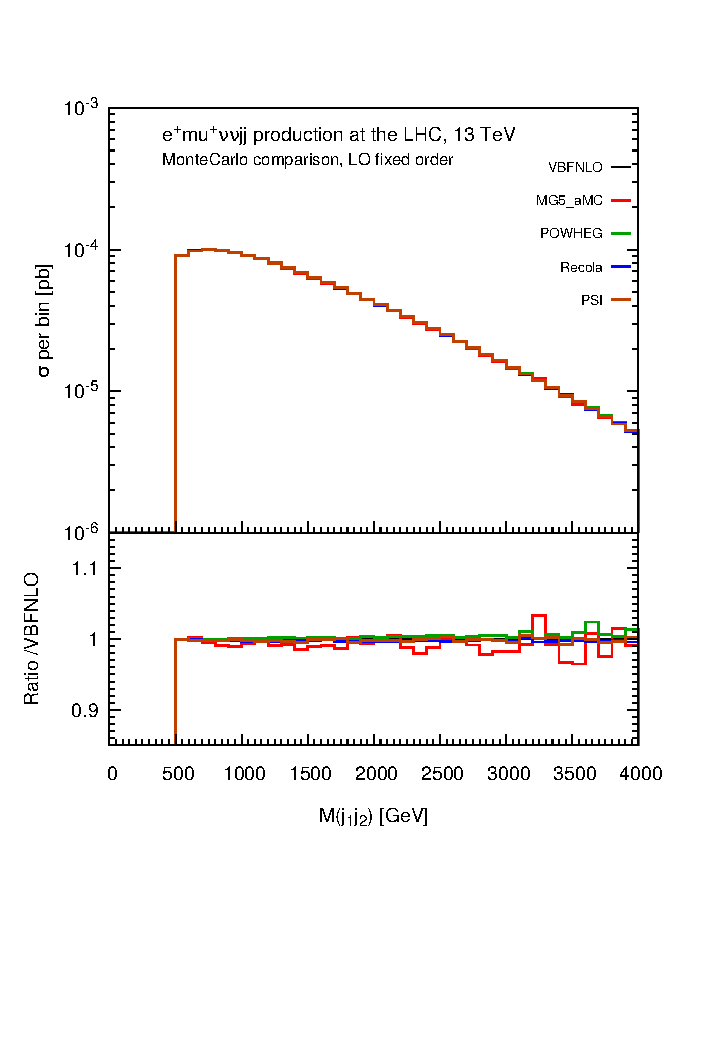
\includegraphics[width=0.49\textwidth,angle=0,clip=true,trim={0.4cm 4.cm 0.6cm 1.5cm}]{figures/mjj_LO.pdf}
   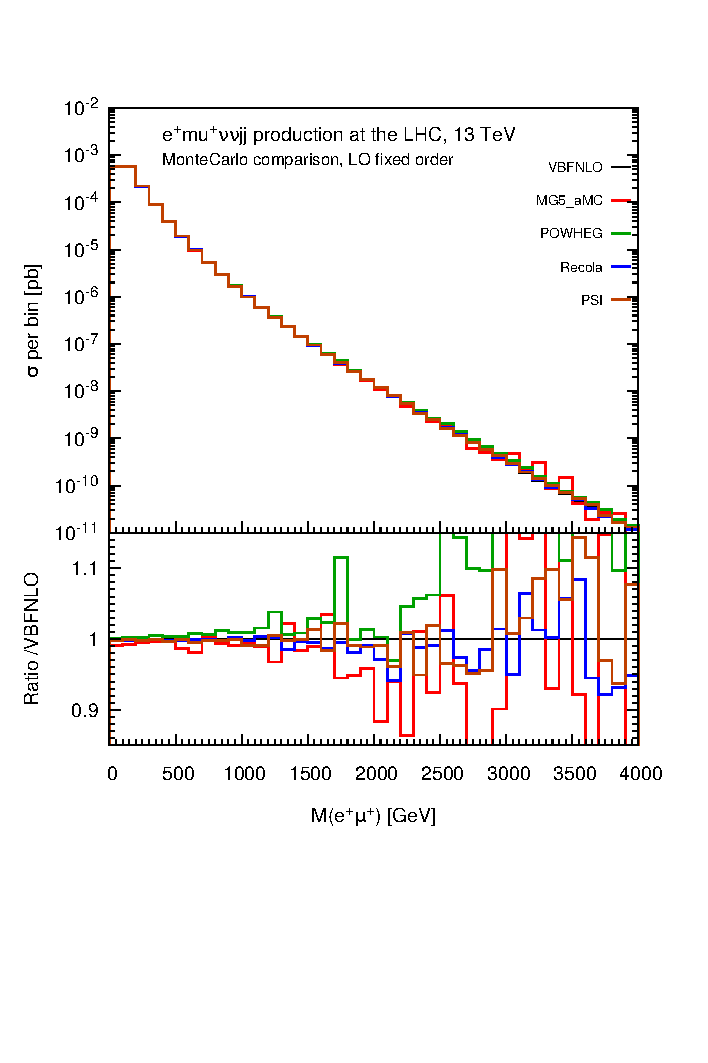
\includegraphics[width=0.49\textwidth,angle=0,clip=true,trim={0.4cm 4.cm 0.6cm 1.5cm}]{figures/mll_LO.pdf}
\caption{\label{fig:mjj-llLO}Invariant-mass of the two tagging jets (left) and of the two leptons (right), at LO.
}
\end{figure}
%
\begin{figure}[h!]
   \centering
   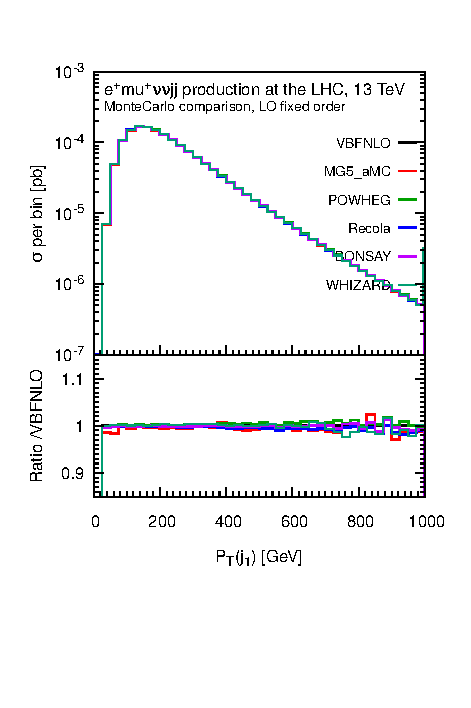
\includegraphics[width=0.49\textwidth,angle=0,clip=true,trim={0.4cm 4.cm 0.6cm 1.5cm}]{figures/ptj1_LO.pdf}
   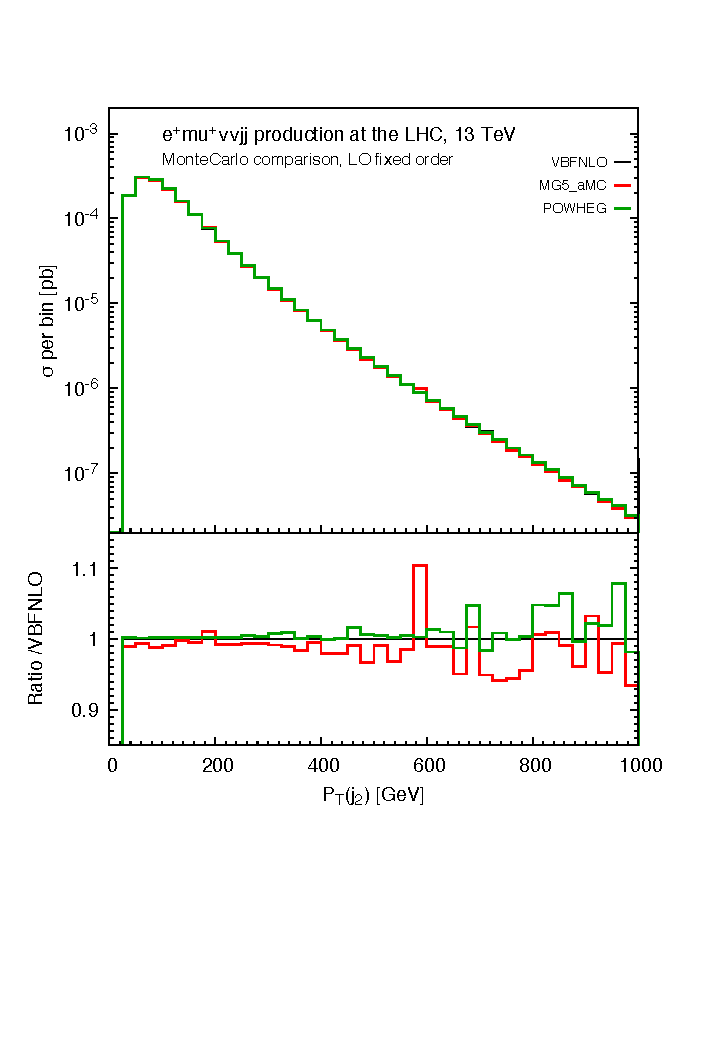
\includegraphics[width=0.49\textwidth,angle=0,clip=true,trim={0.4cm 4.cm 0.6cm 1.5cm}]{figures/ptj2_LO.pdf}
\caption{\label{fig:ptj1-2LO}Transverse momentum of the first (left) and second (right) tagging jet, at LO.
}
\end{figure}
%
\begin{figure}[h!]
   \centering
   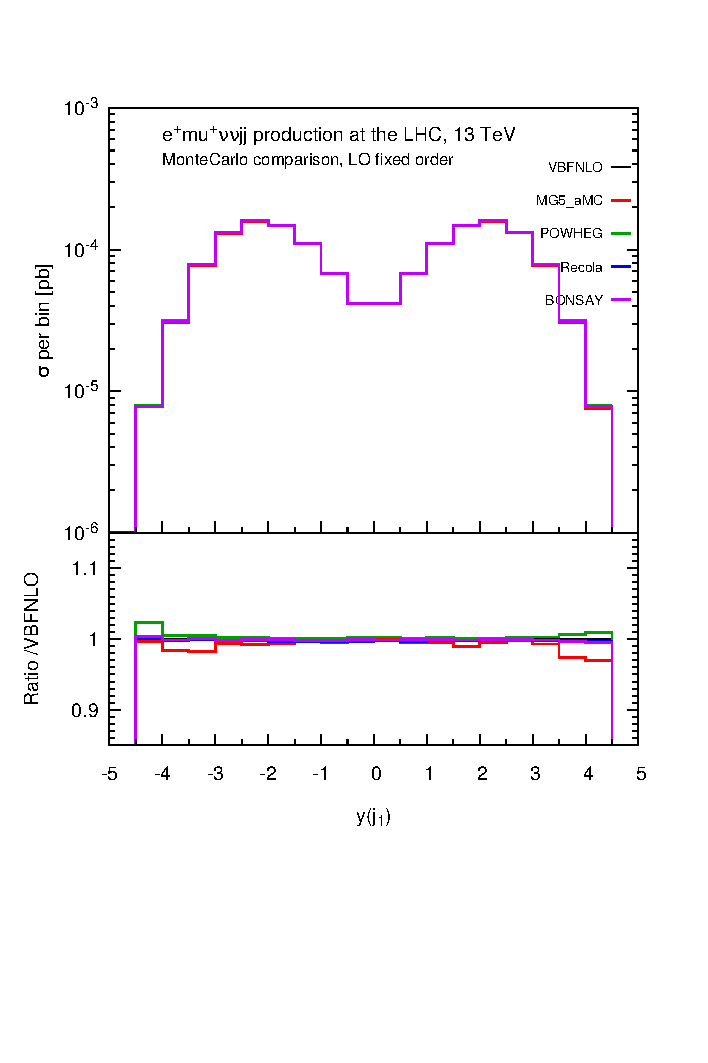
\includegraphics[width=0.49\textwidth,angle=0,clip=true,trim={0.4cm 4.cm 0.6cm 1.5cm}]{figures/yj1_LO.pdf}
   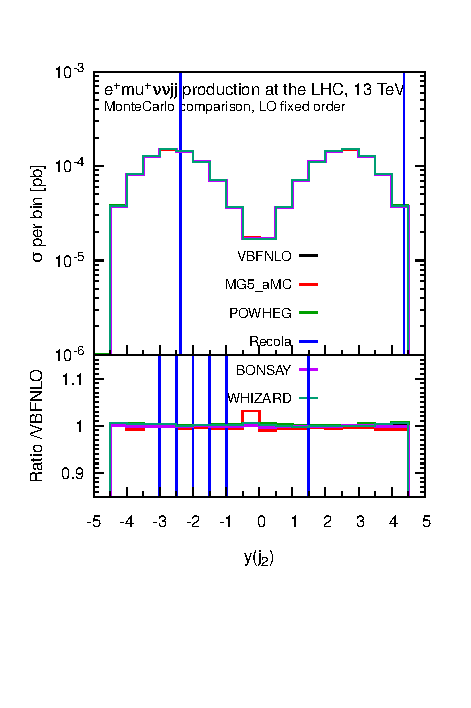
\includegraphics[width=0.49\textwidth,angle=0,clip=true,trim={0.4cm 4.cm 0.6cm 1.5cm}]{figures/yj2_LO.pdf}
\caption{\label{fig:yj1-2LO}Rapidity of the first (left) and second (right) tagging jet, at LO.
}
\end{figure}
%
\begin{figure}[h!]
   \centering
   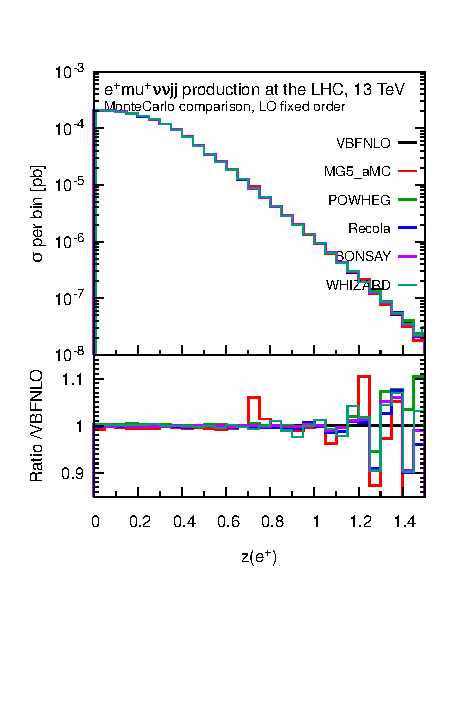
\includegraphics[width=0.49\textwidth,angle=0,clip=true,trim={0.4cm 4.cm 0.6cm 1.5cm}]{figures/ze_LO.pdf}
   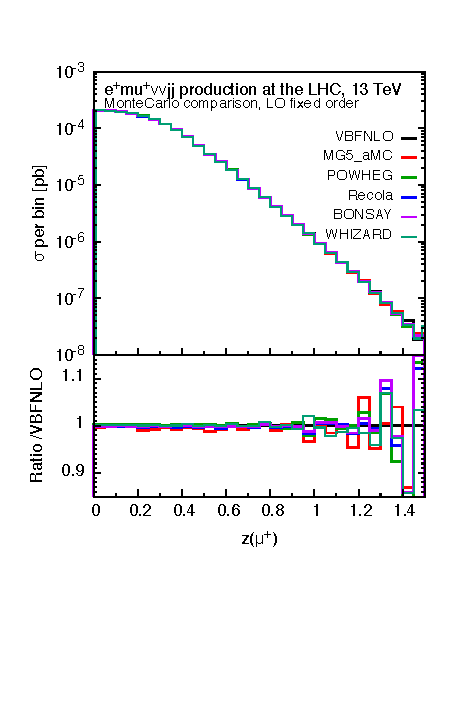
\includegraphics[width=0.49\textwidth,angle=0,clip=true,trim={0.4cm 4.cm 0.6cm 1.5cm}]{figures/zmu_LO.pdf}
\caption{\label{fig:zel-muLO}Zeppenfeld variable of the positron (left) and of the muon (right), at LO.
}
\end{figure}



\subsection{NLO $\mathcal{O}\left(\alpha^6\alpha_{\rm s}\right)$}

\begin{table}[h!]
    \begin{tabular}{c|c|c|c}
        Code  &  $\sigma[\rm{fb}]$  &  $\sigma(n_j=2)[\rm{fb}]$  &  $\sigma(n_j=3)[\rm{fb}]$\\
        \hline
        \hline
        {\sc POWHEG}  &  \\
        {\sc Recola}  &  \\
        {\sc VBFNLO}  &  $1.3531 \pm 0.0003$  &  $0.8264 \pm  0.0003$  &  $0.5267 \pm 0.0001$\\
        Private       &  \\
        {\sc MG5\_aMC}&  $1.315 \pm 0.003$  &  $0.784 \pm  0.003$  &  $0.5313 \pm 0.0009$\\
    \end{tabular}
    \caption{\label{tab:NLOrates} NLO rates within VBS cuts from the different codes.}
\end{table}

\begin{figure}[h!]
   \centering
   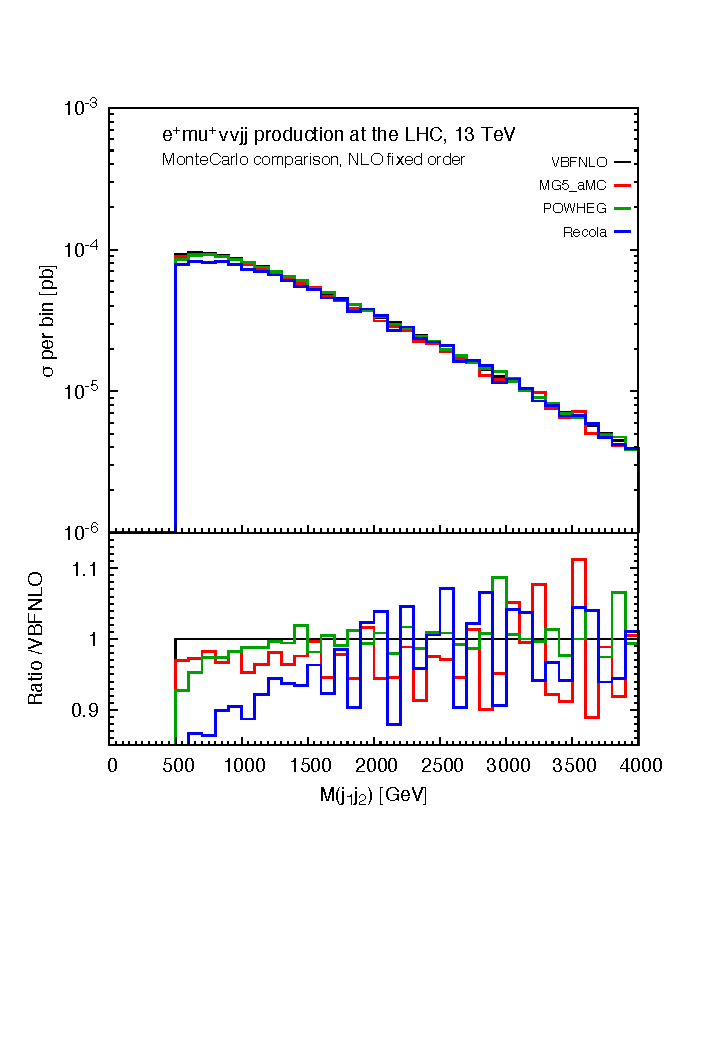
\includegraphics[width=0.49\textwidth,angle=0,clip=true,trim={0.4cm 4.cm 0.6cm 1.5cm}]{figures/mjj_NLO.pdf}
   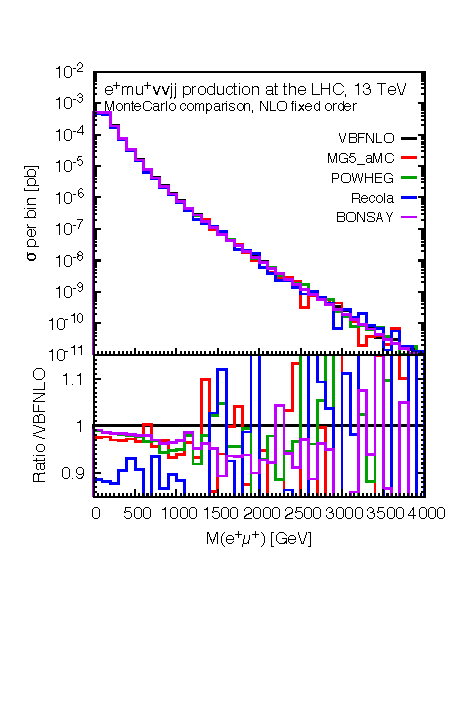
\includegraphics[width=0.49\textwidth,angle=0,clip=true,trim={0.4cm 4.cm 0.6cm 1.5cm}]{figures/mll_NLO.pdf}
\caption{\label{fig:mjj-llNLO}Invariant-mass of the two tagging jets (left) and of the two leptons (right), at NLO.
}
\end{figure}
%
\begin{figure}[h!]
   \centering
   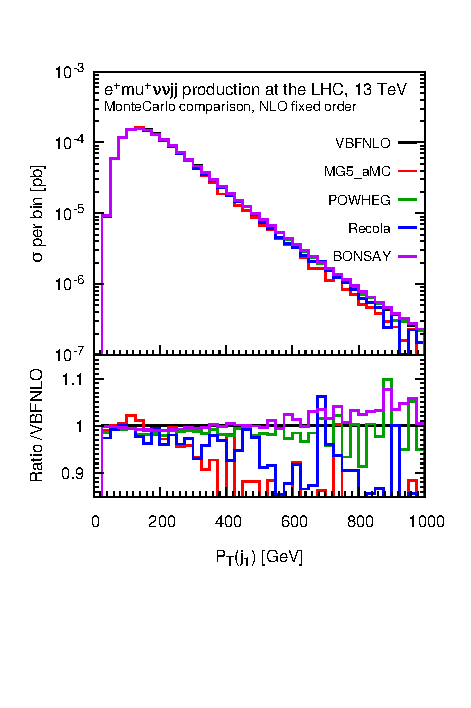
\includegraphics[width=0.49\textwidth,angle=0,clip=true,trim={0.4cm 4.cm 0.6cm 1.5cm}]{figures/ptj1_NLO.pdf}
   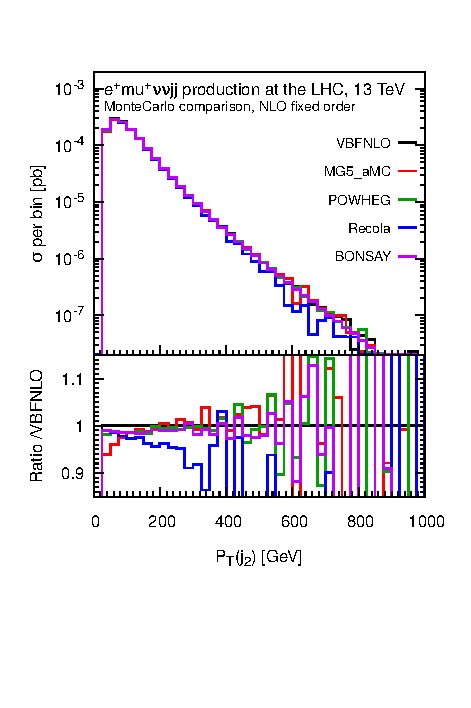
\includegraphics[width=0.49\textwidth,angle=0,clip=true,trim={0.4cm 4.cm 0.6cm 1.5cm}]{figures/ptj2_NLO.pdf}
\caption{\label{fig:ptj1-2NLO}Transverse momentum of the first (left) and second (right) tagging jet, at NLO.
}
\end{figure}
%
\begin{figure}[h!]
   \centering
   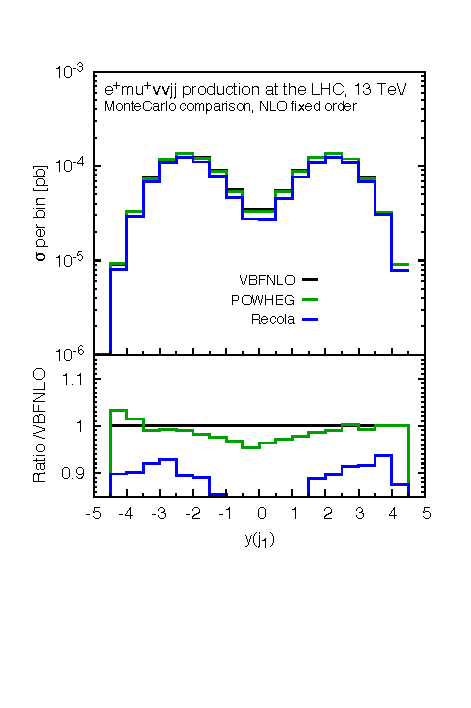
\includegraphics[width=0.49\textwidth,angle=0,clip=true,trim={0.4cm 4.cm 0.6cm 1.5cm}]{figures/yj1_NLO.pdf}
   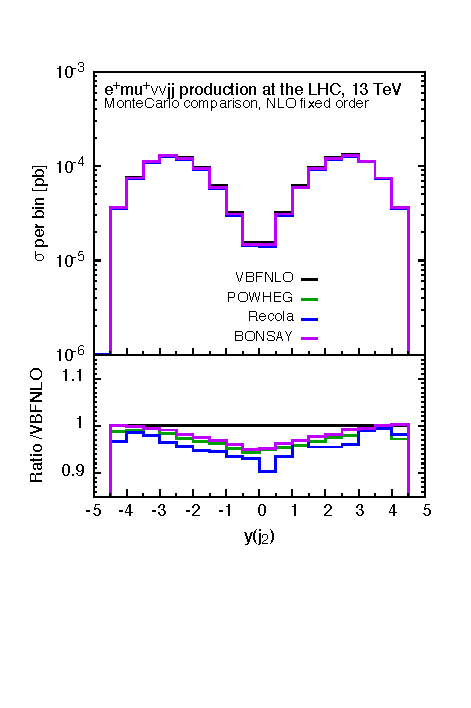
\includegraphics[width=0.49\textwidth,angle=0,clip=true,trim={0.4cm 4.cm 0.6cm 1.5cm}]{figures/yj2_NLO.pdf}
\caption{\label{fig:yj1-2NLO}Rapidity of the first (left) and second (right) tagging jet, at NLO.
}
\end{figure}
%
\begin{figure}[h!]
   \centering
   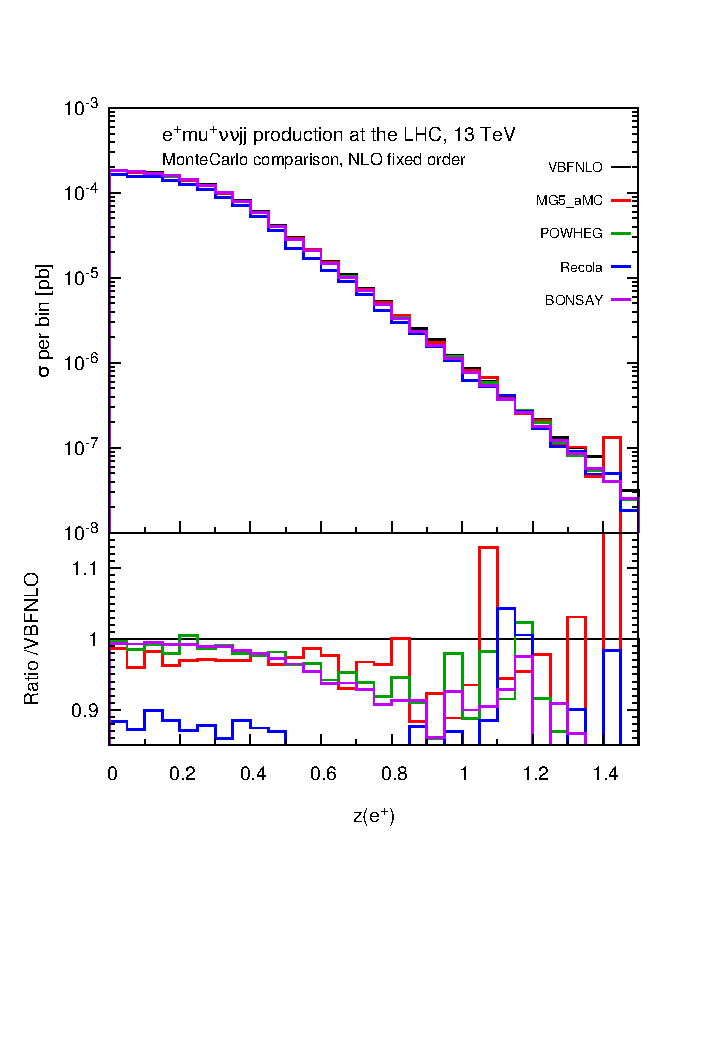
\includegraphics[width=0.49\textwidth,angle=0,clip=true,trim={0.4cm 4.cm 0.6cm 1.5cm}]{figures/ze_NLO.pdf}
   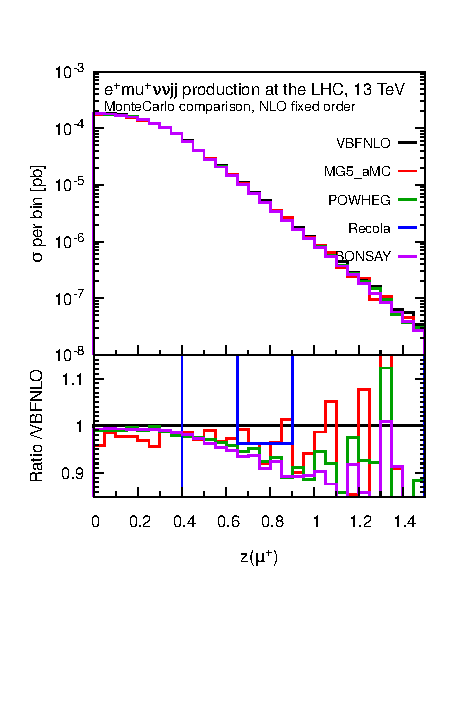
\includegraphics[width=0.49\textwidth,angle=0,clip=true,trim={0.4cm 4.cm 0.6cm 1.5cm}]{figures/zmu_NLO.pdf}
\caption{\label{fig:zel-muNLO}Zeppenfeld variable of the positron (left) and of the muon (right), at NLO.
}
\end{figure}

\part{Conclusion}

\part{Acknowledgments}

Karlsruhe for hosting the documents used for the comparison.

\end{document}          
